Je ne l'ai découvert que trop tard, mais durant la blackhat 2016, s'est déroulée une présentation sur le sujet du stage \footnote{\url{https://www.blackhat.com/docs/us-16/materials/us-16-Yoon-Attacking-SDN-Infrastructure-Are-We-Ready-For-The-Next-Gen-Networking.pdf}}. Cette présentation résume les différents points névralgiques d'ONOS et d'OpenDayLight, et les schémas y sont limpides (pour les lecteurs désirant bien se figurer certaines attaques). 

Parmi les principales attaques qui n'ont pas encore été évoquées, on trouve :

\begin{list}{$\Asteriscus$}{}

\item les attaques sur les switchs : si ceux-ci n'implémentent pas correctement le protocole Openflow ou sont faiblement configurés et qu'il est possible d'en prendre le contrôle, on se retrouve dans le cas où on peut plus facilement exécuter les attaques précédentes sur l'interface sud d'homme au milieu et de deni de service.

\item les attaques liées à la gestion multi-contrôleurs éventuelle : il existe une possibilité de contrôler un switch depuis plusieurs contrôleurs à la fois (par exemple pour assurer le service si un contrôleur tombe en panne) et également une possibilité d'échange d'informations entre contrôleurs. Or il n'existe pas encore ni de mécanisme standardisé ni de sécurité très élevée pour de tels échanges, et la capacité des switchs à être contrôlés par plusieurs contrôleurs repose sur la notion de contrôleurs maître/esclaves qui peut aboutir à un deni de service si un contrôleur malveillant monopolise le rôle de maître sur un switch (sans parler des vulnérabilités existantes sur les switchs qui permettent même en étant un contrôleur esclave de modifier les tables de flux \footnote{Un collègue à Telecom Sudparis a travaillé sur ce point et montré la vulnérabilité sur certains switchs}).

\item les attaques sur le plan de communication : comme on l'a déjà dit, sans TLS, pas de confidentialité ni de confiance dans les données qui transitent via Openflow et donc possibilité pour un attaquant situé dans le réseau de prendre le contrôle d'une partie de celui-ci et de créer des messages malicieux dirigés contre le contrôleur. Mais l'activation de TLS avec authentification mutuelle n'est pas évidente à mettre en place (PKI fiable, qui puisse assurer la révocation, ...).

\item les attaques sur les environnements de développement et de déploiement : lors de la construction du contrôleur avec maven le code mais aussi d'autres éléments nécessaires peuvent être (et le sont même dans tous les cas réels) obtenus de manière distante sur des dépôts externes. Si la machine utilisée est corrompue (fichiers de configurations modifiés, DNS cache poisoning, ARP spoofing, malware, ...) alors toute l'installation qui en découle sur les contrôleurs peut fournir une opportunité énorme à l'attaquant de contrôler l'ensemble du réseau. C'est une menace très importante en terme d'impact et dont la probabilité n'est pas si faible qu'on pourrait le penser (social engineering, concentration des efforts sur une seule cible).

\item les attaques sur les stations de contrôle et d'administration : vu que certains éléments du conteneur OSGi d'ONOS permettent d'obtenir des droits importants sur le réseau, il est, comme sur un réseau classique, crucial de bien protéger les machines utilisées pour l'administration (là encore le social engineering peut être utilisé).

\end{list}

Pour bien mettre en valeur les spécificités éventuelles d'ONOS, le tableau suivant récapitule impacts et parades des différentes catégories d'attaque qu'on est susceptible de retrouver.

\begin{small}

\begin{longtable}{| p{.26\textwidth} | p{.37\textwidth} | p{.37\textwidth}|}

\hline
\textbf{Catégorie\newline d'attaque et spécificité} & \textbf{Impact} & \textbf{Parade} \\
\hline
Flux réseaux forgés \newline -non spécifique SDN \newline -non spécifique ONOS & Injection de trafic pouvant conduire à du DoS ou de l'homme au milieu avec des conséquences plus grandes que sur un réseau classique & Programmation intelligente du contrôleur\\ 
\hline
Vulnérabilités sur les \newline switchs \newline -non spécifique SDN \newline -non spécifique ONOS & Attaque directe sur les switchs pouvant là encore avoir des conséquences plus grandes que sur un réseau classique à cause des communications avec le contrôleur & TLS avec authentification mutuelle au niveau du plan de contrôle pour diminuer l'impact d'une prise de contrôle d'un switch, ou modèle de confiance à implémenter\\ 
\hline
Vulnérabilités sur les communications au niveau du plan de contrôle \newline -spécifique SDN \newline -non spécifique ONOS &  Si TLS n'est pas activé, ou si c'est une version vulnérable qui est utilisée, ou si la gestion des certificats est faible, impact significatif sur le réseau en cas d'entité malveillante connectée (possibilité de modifier du trafic réseau local et de falsifier les informations demandées par le contrôleur) & Duplication de contrôleurs, modèle de confiance oligarchique (ordre accepté uniquement si il est reçu en provenance de plusieurs sources). A noter que cela reste théorique (ça n'est pas encore implémenté ni prévu dans le protocole Openflow)\\ 
\hline
\textbf{Vulnérabilités sur le\newline contrôleur (ONOS)} \newline -spécifique SDN \newline -spécifique ONOS \newline Point le plus important & Compromission totale du réseau en cas de compromission du contrôleur, possibilité de nuisance proportionelle à l'offre fournie en matière d'exécution de code (plusieurs niveaux de compromission : au sein du contrôleur avec un accès plus ou moins restreint au système, puis compromission de la machine hébergeant le contrôleur, et enfin compromission avec droits administrateurs sur la machine)  & Secure-mode obligatoire !\newline Restrictions des interfaces, restrictions des permissions, configuration soigneusement effectuée (CLI, GUI, ssh, options du contrôleur). Duplication des contrôleurs et mécanismes de restauration à prévoir\\ 
\hline
Manque de confiance entre contrôleur et applications \newline -spécifique SDN \newline -non spécifique ONOS & Impact significatif en cas d'application malveillante avec des permissions trop élevées. Danger critique au niveau des dépôts de code externe (code source, ou dépôt maven pour les dépendances) utilisés pour le développement et la mise en production automatique & Applications critiques signées, applications externes avec des permissions peu critiques, mécanismes de log permettant de sauvegarder les appels clés. Signature du code (coeur d'ONOS notamment), mécanismes de protection d'intégrité des fonctions critiques\\ 
\hline
Vulnérabilités sur les stations d'administration \newline -non spécifique SDN \newline -non spécifique ONOS & Impact beaucoup plus élevé que dans un réseau classique (avec les droits d'utilisation de l'API REST par exemple on peut modifier l'intégralité du réseau en téléchargeant une seule application sur le contrôleur) & Politique stricte de gestion des accès (double authentification, peu de personnes autorisées à accéder aux fonctionnalités de l'API REST ...). L'idéal serait qu'ONOS offre le même niveau de séparation des privilèges à ce niveau qu'au niveau applicatif avec le Secure-mode.\newline Mécanismes de restauration en cas d'attaque détectée ou de disfonctionnement majeur\\ 
\hline
Manque de solutions efficaces pour l'analyse forensique \newline -non spécifique SDN \newline -non spécifique ONOS & Ca n'est pas vraiment une attaque mais en cas de problèmes/d'attaque il est nécessaire d'avoir les outils qui permettent une restauration efficace et une compréhension rapide des évènements & Fichiers de logs (concernant les décisions prises au niveau du contrôleur mais aussi les paquets Openflow circulant sur le réseau) indélébiles et stockés de manière sécurisée\\ 
\hline

\end{longtable}

\end{small}

Ainsi, la réplication des contrôleurs permet d'obtenir une redondance qui pallie à certains problèmes (si en plus on place différents responsables avec différents identifiants/clés à la tête de chaque contrôleur, on peut avoir un réseau fonctionnel alors qu'un des contrôleurs est compromis par exemple).\\
Par contre, en mettant en place un tel système, on perd nécessairement en performances puisque les mêmes opérations sont globalement effectuées sur chaque. Et malgré le mode maître/esclave qui permet à un switch de savoir qui est son chef, le protocole Openflow ne prend pas encore en compte un mode multi-contrôleur complexe, donc un switch ne peut pas encore réagir en fonction de la confiance associée à un ordre (si un contrôleur maître envoie un ordre contradictoire par rapport à deux autres, le switch tentera tout de même d'exécuter cet ordre). Pour l'instant la réplication aurait donc tendance à compliquer énormément les choses (d'autant que, si un contrôleur maître est compromis, il peut dans tous les cas agir négativement sur le switch même si il existe d'autres contrôleurs maîtres qui envoient des ordres contraires, provoquant ainsi de toute façon un déni de service).\\
Cela offre toutefois une réflexion intéressante sur un moyen de solutionner l'un des plus gros problèmes des réseaux SDN à l'heure actuelle à savoir l'impact d'une compromission totale du contrôleur.

\begin{figure}[h]
  	\centering
  	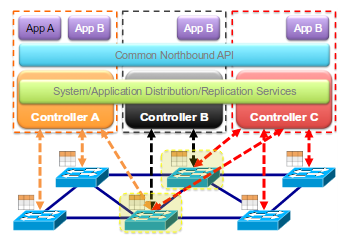
\includegraphics[width=0.5\textwidth]{replication.png}
  	\caption{Réplication des contrôleurs : duplication des ordres, résilience en cas de problème sur un contrôleur}
\end{figure}
